%\addcontentsline{toc}{chapter}{App}
\chapter{Auswertung}
Dieser Teil widmet sich nicht nur das Starten der Anwendung(Partikel-Tracking-System) sondern auch die Auswertung der Ergebnisse bzw. Bilder mit lokalisierten Partikeln aus der Verwendung des Partikelverfolgungssystems, um die Beurteilung des Renderings zu erleichtern.
In diesem Sinne haben wir im Rahmen unserer Arbeit die Python-Bibliothek \textbf{bokeh} verwendet. Diese ermöglicht es, interaktive Visualisierungen für moderne Webbrowser zu erstellen und "hilft dabei, wunderschöne Grafiken zu erstellen, von einfachen Plots bis hin zu komplexen Dashboards mit kontinuierlichen Datensätzen", wie es auf ihrer Website beschrieben wurde \cite{bokeh}.

%\addcontentsline{toc}{section}{App}
\section{App}
Nachdem wir in den vorherigen Abschnitten gesehen haben, wie man die Parameterwerte für das allererste Bild auswählt und die wichtigsten Methoden der Anwendung wie \textit{update\_frame} und \textit{get\_particle\_per\_frame} kennengelernt haben, ist es uns wichtig zu zeigen, wie man die Anwendung startet und wo man was einsetzt, um sie zu benutzen.
Entsprechend werden wir uns im nächsten Abschnitt mit der Installation des Systems befassen.

\subsection{Installation}
Zuerst müssen Sie sich das Paket besorgen. Sie können das Projekt entweder aus dem github-Repository \cite{particleTrackingSystem} klonen oder es einfach downloaden. Sobald das Repository lokal auf Ihrem Computer verfügbar ist, ist der nächste Schritt, sich eine IDE zu besorgen. Es ist zwar möglich, das Projekt über das Terminal zu starten, aber wir empfehlen dringend die Verwendung einer IDE, vorzugsweise PyCharm.\\
Danach müssen Sie nur noch das Repository mit dem von Ihnen gewählten Editor öffnen.  
Da die Installation des Systems größtenteils auf der Installation von Trackpy basiert, die in \ref{Kap2.1_Einleitung_Installation} durchgeführt wurde, müssen Sie zuerst die Schritte zur Installation von Trackpy befolgen und anschließend unbedingt auch "bokeh" installieren.   
Wie auf ihrer Seite beschrieben, können wir je nach Arbeitsumgebung entweder \textsl{\textbf{conda install bokeh}} für eine conda-Umgebung oder \textsl{\textbf{pip install bokeh}} verwenden (\textit{siehe} \cite{bokeh}).
Nach der Installation ist das System betriebsbereit und einsatzbereit.

\subsection{Bedienung der Anwendung}
\begin{enumerate}
	\item \textbf{Backendseitig}\\
	Nach der erfolgreichen Installation müssen Sie in die Datei \textbf{ParticleTrackingSystem/launcher.py} gehen, die hauptsächlich zur Ausführung der Funktionen dient, die hier zur Verfügung gestellt werden. Die Funktion "\textbf{set\_path}", die im Programm beschrieben wird, ermöglicht es, den Ort der Datei anzugeben, genauer gesagt den Ort des Videos, das wir auf die Bewegung der vorhandenen Partikel untersuchen wollen. 
Mit Hilfe der Variable "\textbf{tracker}", die nichts anderes als ein Objekt vom Typ \textbf{Tracker} ist, müssen wir ihr jeweils die Elemente zuweisen, die sie wissen muss:
\begin{itemize}
   \item Den Durchmesser der Partikel über den Konstruktor
   
   \item Die zu manipulierende Bildsequenz (wird automatisch erstellt).
   
   \item Die Minmasse der Partikel.
   
   \item Schließlich die Trennung
\end{itemize}

Alle Werte sollten aus dem ersten Bild oder einem Modellbild gemäß \ref{kap3_OP} ausgewählt werden.\\
Anschließend kann man den maximalen und minimalen Prozentsatz der zu findenden Partikel festlegen.\\
Wenn Sie all dies getan haben, müssen Sie nur noch die Datei \textbf{launcher.py} ausführen und einige Sekunden warten, bis das Programm ausgeführt wird. Dies ist alles für die Ausführung des Programms. Jetzt müssen wir nur noch die Visualisierung (Frontend) über Bokeh starten.
	\item \textbf{Frontendseitig}\\
	Das Frontend lässt sich starten, indem man ein Terminal öffnet, in das \textbf{ParticleTrackingSystem} wechselt und dort den folgenden Befehl ausführt:\\ \textbf{python -m bokeh serve --show .$\setminus$ParticleTrackingSystem$\setminus$}. \\ Es erscheint eine Seite mit einem Button, der eine Diashow der Bilder mit den lokalisierten Partikeln und den Werten der angewandten Parameter, die zu dem zu sehenden Ergebnis geführt haben, startet.
	
	\begin{figure}[H]
    \centering
    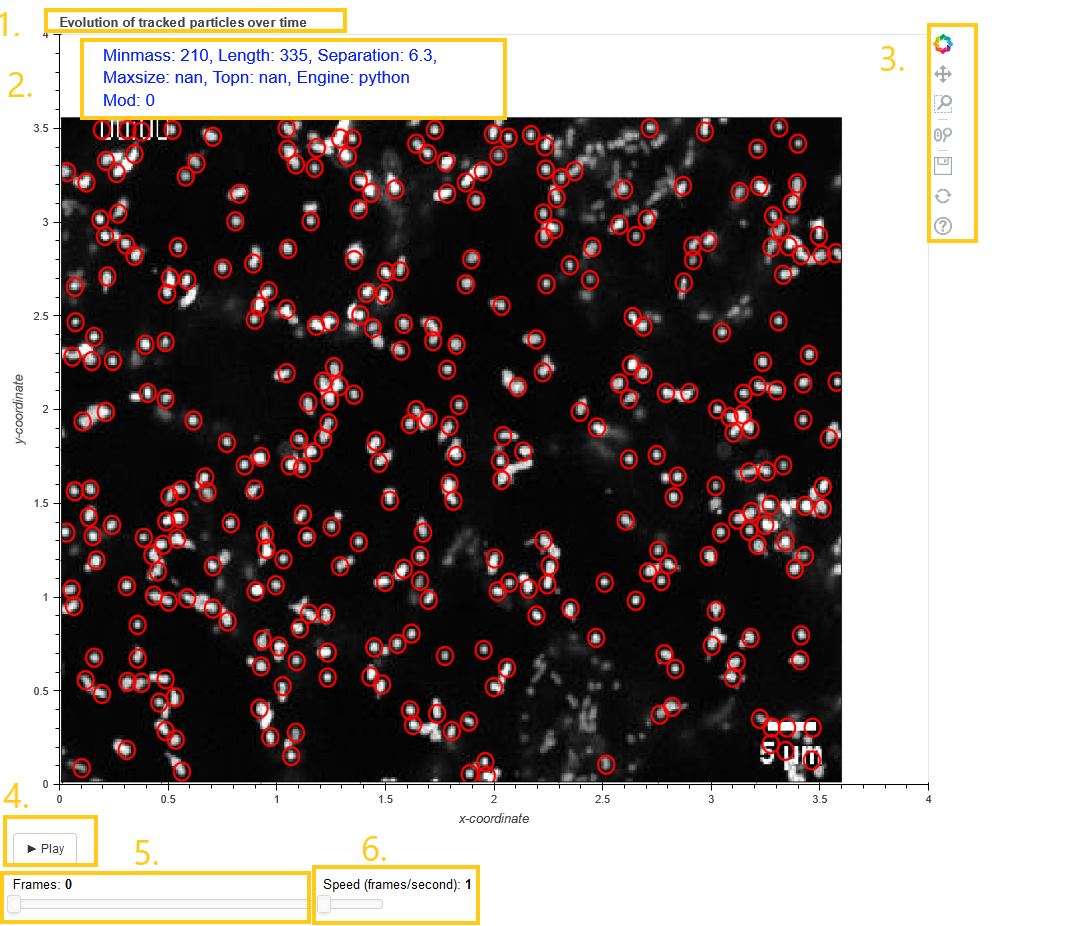
\includegraphics[scale=0.5]{Grafiken/bokeh/GUI presentation.png}
    \caption{Frontend presentation}
    \label{fig:kap_App/GUI presentation}
\end{figure} 

\begin{tabular}{|l|p{12cm}|}
\hline
\texttt{1.} & Titel der Seite (bleibt unverändert). \\ \hline
\texttt{2.} & Parameterwerte, die zum Ergebnis geführt haben ($+$ length). \\ \hline
\texttt{3.} & Von Bokeh bereitgestellte Tools (Zoomen, Verschieben, Speichern und Neuladen, ...). \\ \hline
\texttt{4.} & Play- und Pause-Button zum Starten und Pausieren der Diashow. \\ \hline
\texttt{5.} & Zeigt den Frame an, in dem man sich gerade befindet, und ermöglicht es, zu einem anderen Frame zu wechseln. \\ \hline
\texttt{6.} & Reguliert die Reihenfolge der Bilder (z. B. Bild nach Bild oder jedes zweite Bild). \\ \hline
\hline
\end{tabular}
\\ \\

Sollte das Ergebnis (eines bestimmten Bildes) nicht zufriedenstellend sein, kann es mit der Funktion \textit{update\_frame}, wie im vorherigen Kapitel beschrieben, geändert werden. Allerdings muss der Bokeh-Server nach der Änderung neu gestartet werden, um sicherzustellen, dass das neue Bild und seine Parameter angezeigt werden können. 
	
\end{enumerate}

%\addcontentsline{toc}{section}{Experimente \& Umsetzung}
%\section{Experimente \& Umsetzung}


%\section{Herausforderungen \& Probleme}